\documentclass[11pt,a4paper]{article}
\usepackage[T1]{fontenc}
\usepackage[utf8]{inputenc}
\usepackage{lmodern,microtype,amsmath,amssymb,graphicx,booktabs,needspace}
\usepackage[margin=24mm,headheight=15pt]{geometry}
\usepackage{xcolor,parskip,fancyhdr,hyperref}
\definecolor{ink}{HTML}{192532}\definecolor{navy}{HTML}{1F4874}\definecolor{muted}{HTML}{52677B}
\hypersetup{colorlinks=true,urlcolor=navy,linkcolor=navy,pdftitle={Inhibitory Interactions in Financial Event Streams},pdfauthor={Imad Jboub, Thomas Nussbaum, Sarah Pouliquen, Hugo Wei, Ayman Zbiri}}
\pagestyle{fancy}\fancyhf{}\fancyhead[L]{\footnotesize\color{muted} RESEARCH ARCHIVE / 2024 PROJECT}\fancyhead[R]{\footnotesize\color{muted} H. WEI}\fancyfoot[C]{\footnotesize\thepage}
\renewcommand{\headrulewidth}{0.35pt}
\newcommand{\sect}[1]{\par\needspace{5\baselineskip}\vspace{1mm}\noindent{\large\bfseries\color{navy}#1}\par\vspace{0.5mm}}
\begin{document}
{\color{navy}\sffamily\bfseries\small RESEARCH SYNOPSIS\quad / \quad EDITORIAL EDITION 2026}\par\vspace{5mm}
{\fontsize{28}{33}\selectfont\bfseries\color{ink} Inhibitory Interactions\\ in Financial Event Streams}\par\vspace{4mm}
{\large Multivariate Hawkes processes, calibration, and parameter identifiability}\par\vspace{5mm}
\hrule\vspace{4mm}
{\small \textbf{Original group report:} Mod\'elisation des ph\'enom\`enes d'inhibition sur les march\'es financiers (8 June 2024).\\
\textbf{Authors:} Imad Jboub, Thomas Nussbaum, Sarah Pouliquen, Hugo Wei, Ayman Zbiri.\\
\textbf{Academic supervisor:} Ioane Muni Toke. \textbf{Institution:} CentraleSup\'elec / MICS.}\par
\sect{Research question}
Can a multivariate point process with both positive and negative interactions describe and calibrate the timing of different order-book event types? How does the assumed decay rate affect parameter recovery and the geometry of the likelihood?
\sect{Mathematical model}
For event types $i=1,\ldots,d$, with counting processes $N_j$, baseline rates $\mu_i>0$, interaction amplitudes $\alpha_{ij}\in\mathbb R$ and decay rates $\beta_{ij}>0$, the model uses a rectified conditional intensity
\begin{equation}
 \lambda_i(t)=\left[\mu_i+\sum_{j=1}^d\int_{[0,t)}\alpha_{ij}e^{-\beta_{ij}(t-s)}\,\mathrm dN_j(s)\right]_+,\qquad [x]_+=\max(x,0).
\end{equation}
The sign of $\alpha_{ij}$ distinguishes excitation from inhibition. The parameter $\beta_{ij}$ is a \emph{temporal decay rate}, not the CAPM market beta or the sensitivity of a security's return to a market index. For an observed event history over $[0,T]$, the log-likelihood (up to irrelevant conventions) is
\begin{equation}
\ell(\theta)=\sum_{i=1}^d\left[\sum_{k:T_k^{(i)}\le T}\log\lambda_i(T_k^{(i)}-) -\int_0^T\lambda_i(s)\,\mathrm ds\right].
\end{equation}
The compensator must integrate the \emph{rectified} intensity, accounting for intervals in which inhibition drives the latent linear predictor below zero. For the restricted case $\beta_{ij}=\beta_i$ within each target component, the latent predictor evolves exponentially between successive event times; this permits an analytic zero-crossing calculation.
\sect{What the 2024 project examined}
The report considered simulation-based parameter estimation, box-plot comparisons of fitted versus generating parameters, order-book event series in several dimensions, and the effect of varying decay assumptions. Its likelihood-profile diagnostics highlighted weak identification of some decay parameters in the tested configurations. These are methodological observations about the studied samples, not claims of a universally consistent or universally inconsistent estimator.
\begin{figure}[ht]
\centering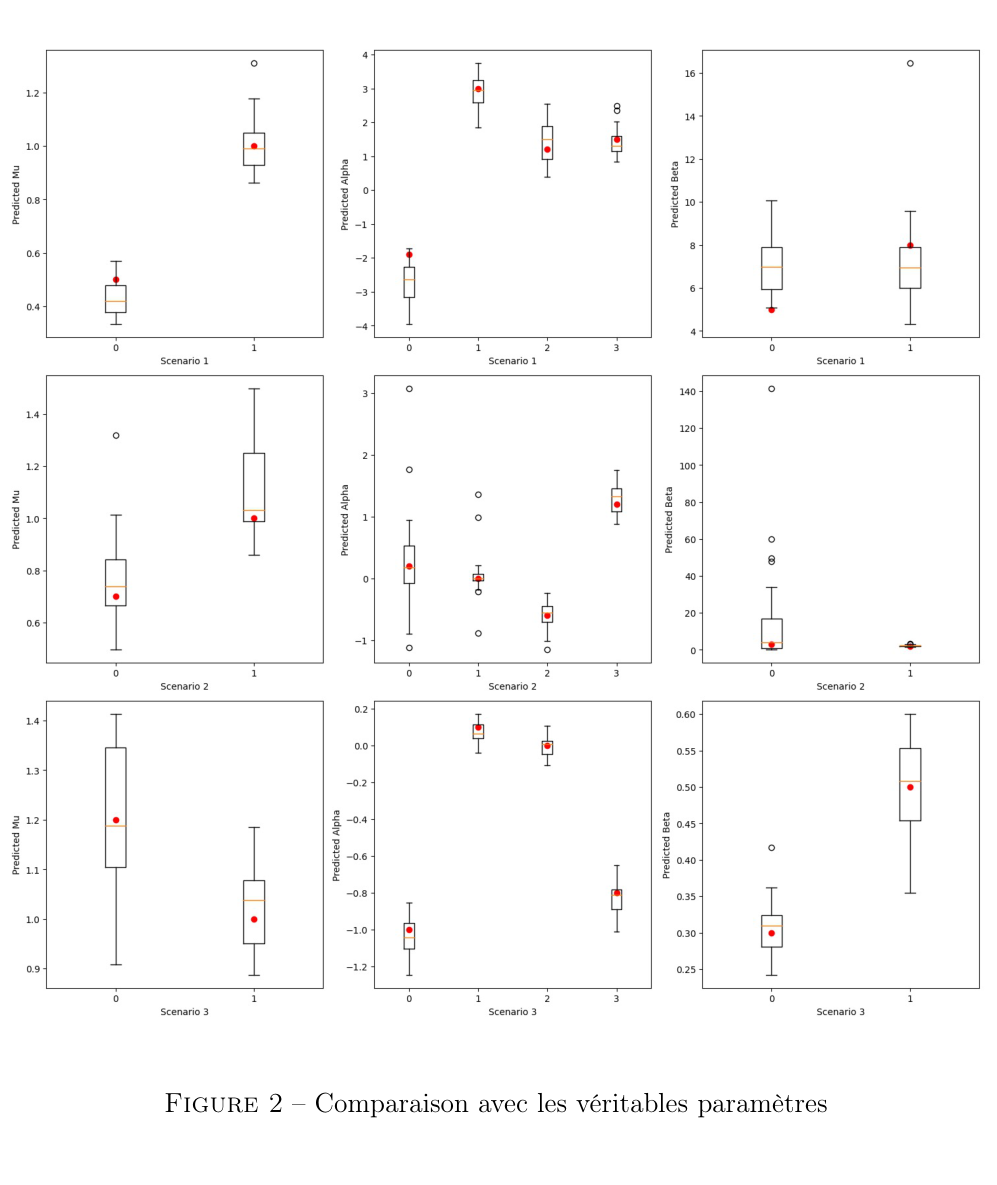
\includegraphics[width=.49\textwidth]{estimation-boxplots.png}
\caption{Parameter-estimation box plots from the 2024 group report (original figure 2). Preserved for historical documentation; the underlying runs have not been independently rerun for this synopsis.}
\end{figure}
\sect{Interpretation and scope}
The study concerns \emph{event intensities}, not a directly simulated stochastic differential equation for asset prices. In particular, parameter-decay changes do not by themselves prove a change in asset-price volatility or forecast performance. A limited set of numerical tests may indicate poor conditioning, whereas general convergence claims require stronger assumptions and a controlled sequence of sample sizes. Figures inherited from the report document the historical analysis; no new empirical or numerical results are asserted here.
\sect{Research relevance}
This project introduced questions that recur in inverse problems: model misspecification, nonlinear likelihood surfaces, distinction between a theoretically identifiable parameter and a numerically stable estimate, and reproducibility of simulation-based calibration.
\sect{Selected references}
\begin{enumerate}\setlength\itemsep{2pt}
\item A. Bonnet, M. Martinez Herrera, and M. Sangnier, ``Inference of multivariate exponential Hawkes processes with inhibition and application to neuronal activity,'' \emph{Statistics and Computing} 33 (2023).
\item X. Lu and F. Abergel, ``High dimensional Hawkes processes for limit order books: modelling, empirical analysis and numerical calibration,'' \emph{Quantitative Finance} 18 (2018).
\end{enumerate}
\end{document}
